\apendice{Manual de especificación de diseño}
\section{Planos}
El montaje inicial consta simplemente de la conexión de la pantalla \textit{LCD} a la \textit{Raspberry Pi} mediante su respectivo \textit{flex} y las conexiones indicadas por el fabricante. Se desarrolló para la prueba del dispositivo portátil y se presenta en la Figura \ref{fig:ras_inicial}.

\begin{figure}[h]
	\centering
    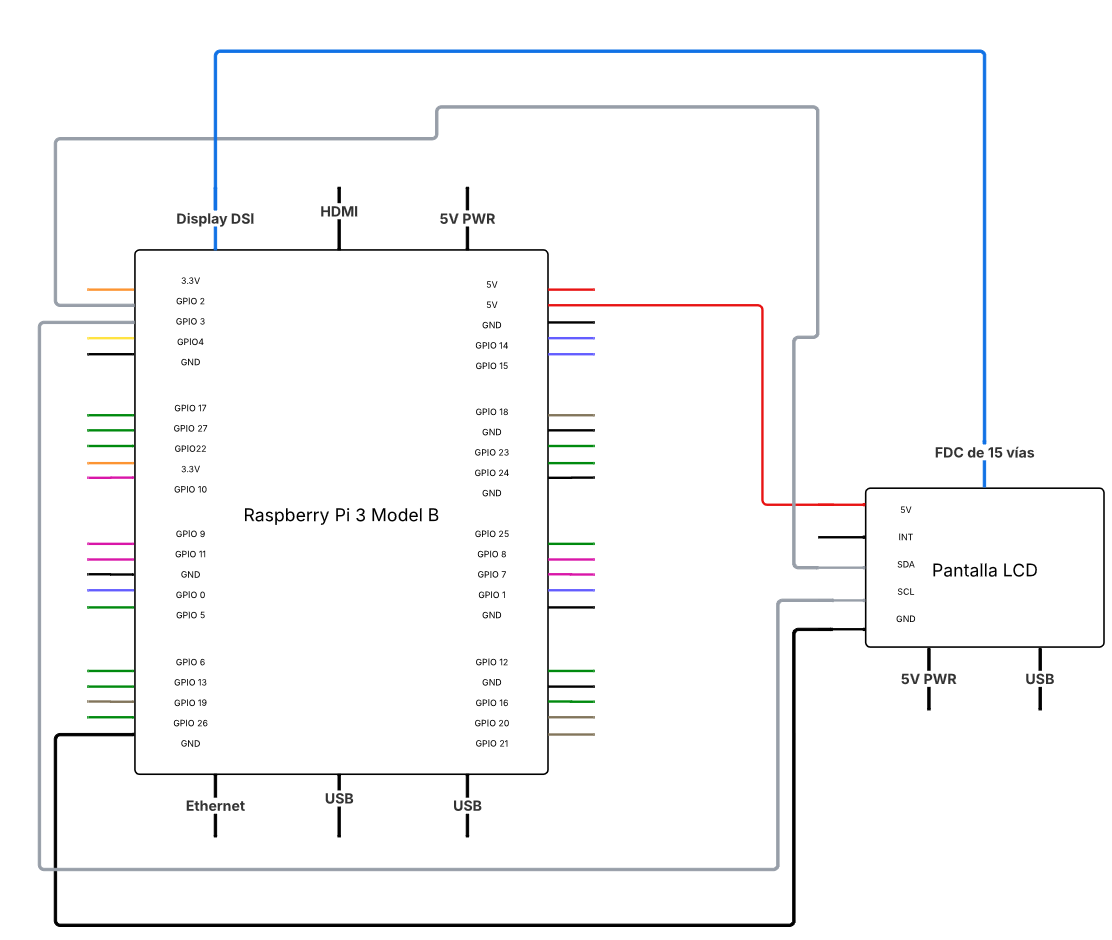
\includegraphics[width=1\textwidth]{img/ras_inicial.png}
    \caption{Montaje inicial para pruebas del prototipo. El esquema de la placa se basa en \cite{diseñorasp}.}
    \label{fig:ras_inicial}
\end{figure}

Tras la comprobación de la viabilidad del dispositivo portátil, se realizaron ciertas mejoras con el objetivos principal de dirigir el dispositivo hacia un enfoque totalmente autónomo. Se implementó una batería de 6000\textit{mAh}, dicho método de almacenamiento, está regulada por un controlador \textit{Adafruit Powerboost 1000C} destinado a la gestión y recarga de la energía del dispositivo. Todo ello emprende gracias a la inclusión de un interruptor \textit{SPDT} conectado al \textit{pin} \textit{EN} del \textit{Poweboost 1000C}. Las conexiones son extremadamente simples, tomando como partida el montaje anterior, solo se necesita conectar el controlador y la pantalla (con su respectivo \textit{flex}) a las fuentes de 5\textit{V} de la placa. Se representa en la Figura \ref{fig:ras_final}.

\begin{figure}[h]
	\centering
    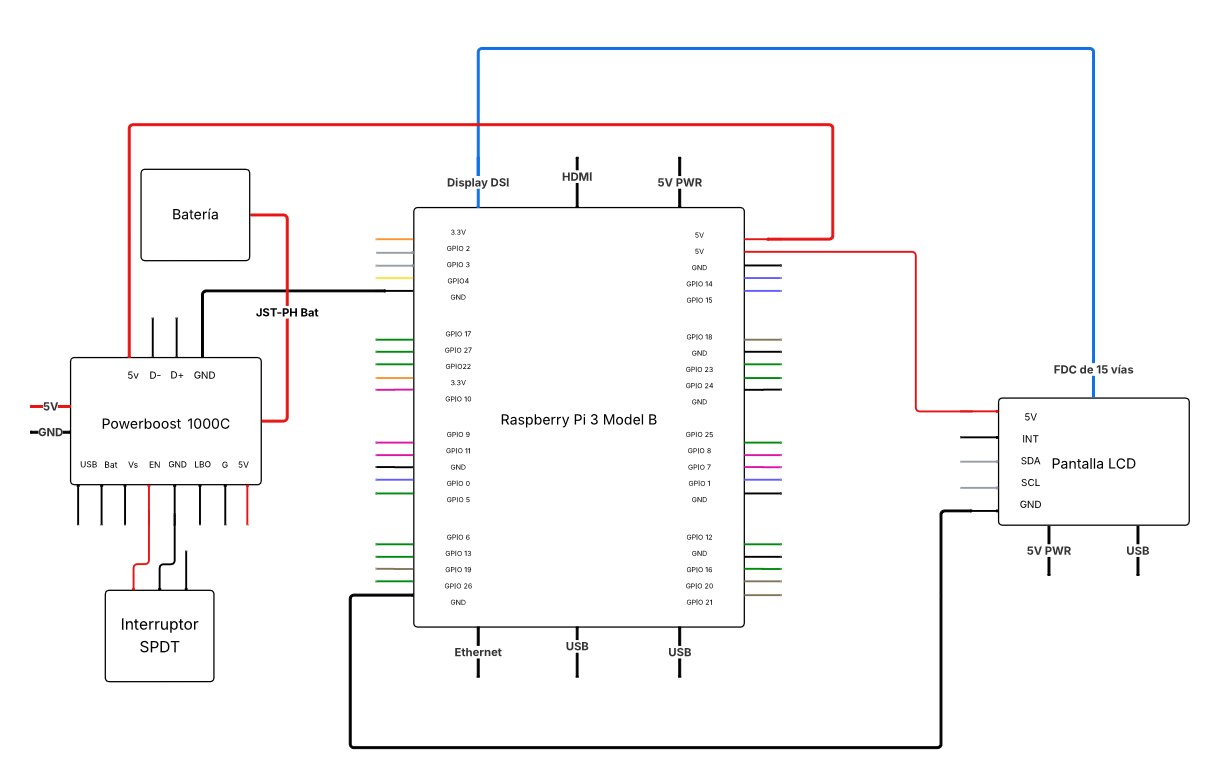
\includegraphics[width=1.2\textwidth]{img/ras_final.png}
    \caption{Esquema del montaje final.}
    \label{fig:ras_final}
\end{figure}

El prototipo final, ilustrado en la Figura \ref{fig:prototipo}, integra todos los componentes de \textit{hardware} esenciales para facilitar su manejo.

\begin{figure}[h]
	\centering
    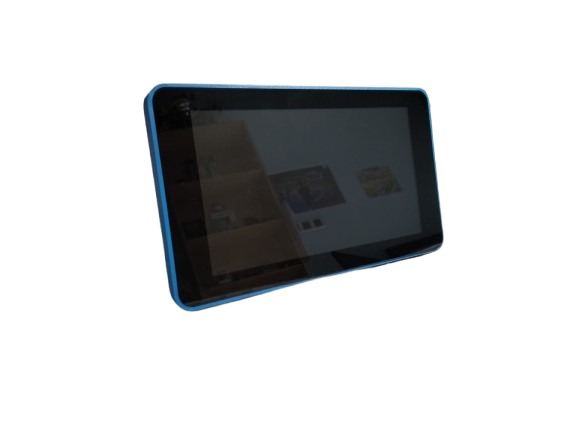
\includegraphics[width=1.2\textwidth]{img/prototipo.png}
    \caption{Prototipo final con todos sus elementos implementados.}
    \label{fig:prototipo}
\end{figure}

\section{Diseño arquitectónico}
Dada la naturaleza colaborativa de la \textit{URCCPQ} y la necesidad de cumplir con la estricta normativa de protección de datos (\textit{LOPD}), la arquitectura de permisos del sistema se ha diseñado bajo un modelo de Control de Acceso Basado en Roles (\textit{RBAC}). A diferencia de los sistemas sin autenticación, esta herramienta implementa una segmentación jerárquica mediante perfiles diferenciados (como \textit{Administrador} y \textit{Facultativo}). Esta decisión técnica, gestionada a través de la base de datos \textit{PostgreSQL}, garantiza que los médicos residentes mantengan un acceso ágil y sin fricciones para la inserción y visualización de registros clínicos, mientras que las operaciones críticas como la exportación masiva del histórico o la gestión de credenciales, quedan restringidas al personal coordinador. De esta forma, se equilibra la operatividad en un entorno de alta demanda con la trazabilidad y la seguridad institucional.

Para documentar la Experiencia de Usuario (\textit{UX}) \cite{ux} y las rutas de navegación de forma clara y legible, se ha descartado la elaboración de un único diagrama de flujo monolítico, el cual resultaría visualmente incomprensible debido a la alta densidad de opciones de la plataforma. En su lugar, el mapa de interacciones se ha estructurado mediante un diseño modular, implementando una distinción semántica específica para clarificar las decisiones: los \textbf{rombos} representan decisiones lógicas automatizadas por el motor del sistema (validaciones de formato, conteo de archivos), mientras que los \textbf{nodos circulares de bifurcación ($\oplus$)} representan los puntos de interacción donde el facultativo médico ejerce una decisión de enrutamiento a través de la interfaz (selección de herramientas o menús). Dividiendo el sistema en los siguientes cinco flujos funcionales de alto nivel:

\begin{itemize}
    \item \textbf{\ref{fig:inicio} - Carga y Validación (Nodo 1):} Constituye la puerta de entrada a la plataforma. El sistema requiere la ingesta de registros ya sean en archivos físicos \textit{CSV} o desde la base de datos. Superadas las validaciones, la información se almacena en la memoria \textit{RAM} del equipo, habilitando el acceso a las tres herramientas analíticas principales (Nodos 2, 3 y 4).
    
    \begin{figure}[h]
		\centering
    		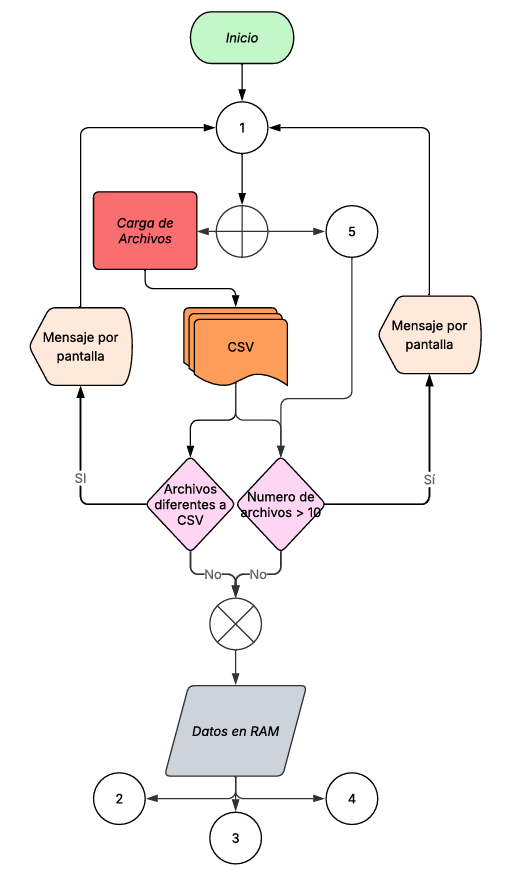
\includegraphics[width=0.6\textwidth]{img/inicio.png}
    		\caption{Diagrama de flujo - Inicio de la \textit{web}.}
    		\label{fig:inicio}
	\end{figure}
    
    \item \textbf{\ref{fig:indicador} - Análisis Individual (Nodo 2):} Este flujo permite al usuario limpiar la sesión o profundizar en un indicador clínico específico. Una vez seleccionado el indicador, el usuario puede bifurcar la visualización hacia un Gráfico Lineal o un Gráfico de Barras, culminando el proceso con la exportación y descarga de los cálculos estadísticos.
    
    \begin{figure}[h]
		\centering
    		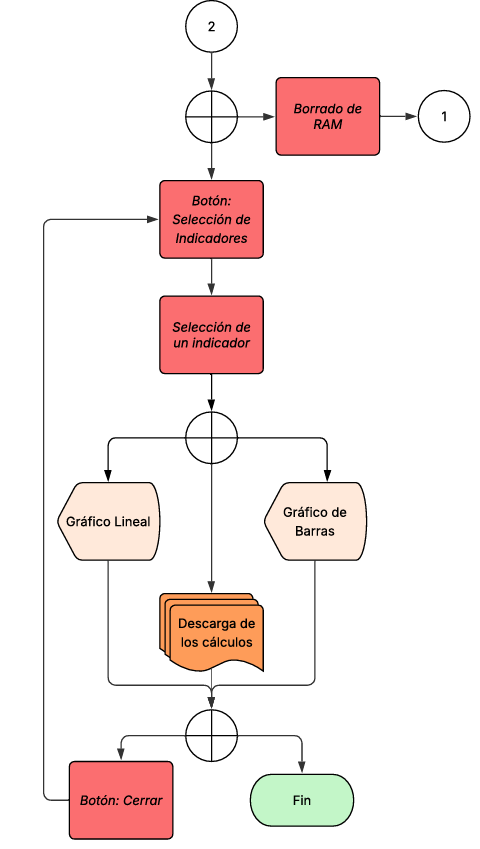
\includegraphics[width=0.6\textwidth]{img/indicador.png}
    		\caption{Diagrama de flujo - Selección de indicadores.}
    		\label{fig:indicador}
	\end{figure}
    
    \item \textbf{\ref{fig:resumen} - Resumen de Indicadores (Nodo 3):} Orientado a la gestión global, esta rama genera un resumen de la unidad clínica. El flujo guía al usuario a través de una tabla resumen y una distribución de ingresos por especialidad médica, permitiendo finalmente descargar el reporte final en formato documento o extraer las tablas específicas.
    
    \begin{figure}[h]
		\centering
    		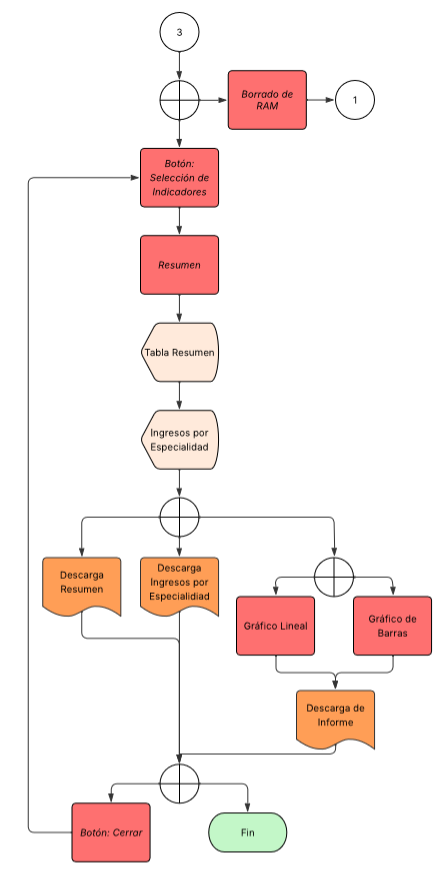
\includegraphics[width=0.6\textwidth]{img/resumen.png}
    		\caption{Diagrama de flujo - Resumen.}
    		\label{fig:resumen}
	\end{figure}
    
    \item \textbf{\ref{fig:mezcla} - Comparativa Avanzada (Nodo 4):} Representa el módulo más complejo de interacción. El flujo \textit{Mezcla} permite al facultativo añadir métricas iterativamente mediante un bucle de control (hasta un máximo de tres indicadores superpuestos) o eliminarlos en tiempo real. Esta iteración finaliza en la selección del tipo de gráfico comparativo, facilitando el análisis cruzado de datos.
    
    \begin{figure}[h]
		\centering
    		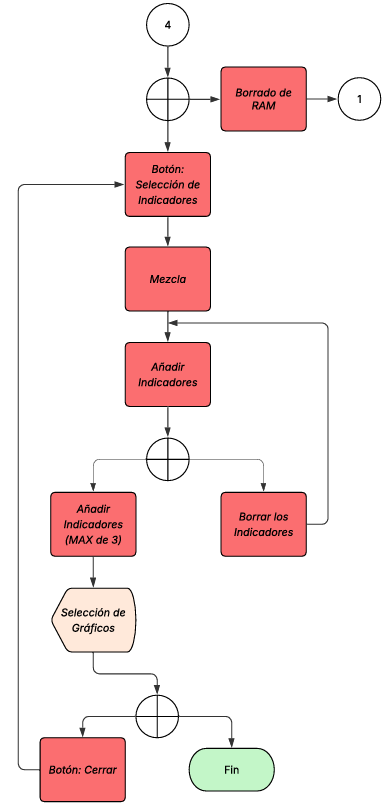
\includegraphics[width=0.6\textwidth]{img/mezcla.png}
    		\caption{Diagrama de flujo - Mezcla.}
    		\label{fig:mezcla}
	\end{figure}
	
	\item \textbf{\ref{fig:bbdd} - Gestión y Persistencia (Nodo 5):} Constituye el núcleo de interacción con el sistema de almacenamiento \textit{PostgreSQL}. A partir de este punto, el flujo lógico se bifurca en tres ramificaciones operativas independientes. La primera permite la adición directa de nuevos registros clínicos al servidor. La segunda ruta exige obligatoriamente una búsqueda previa del paciente, garantizando la consistencia antes de habilitar las funciones de edición o borrado que modifican la base de datos. Finalmente, la tercera ramificación gestiona la consulta del histórico mediante la selección de años, abriendo una nueva compuerta que permite derivar la información hacia dos destinos: su carga volátil en la herramienta para el análisis estadístico, o su exportación masiva, dando por concluido el proceso.
    
    \begin{figure}[h]
		\centering
    		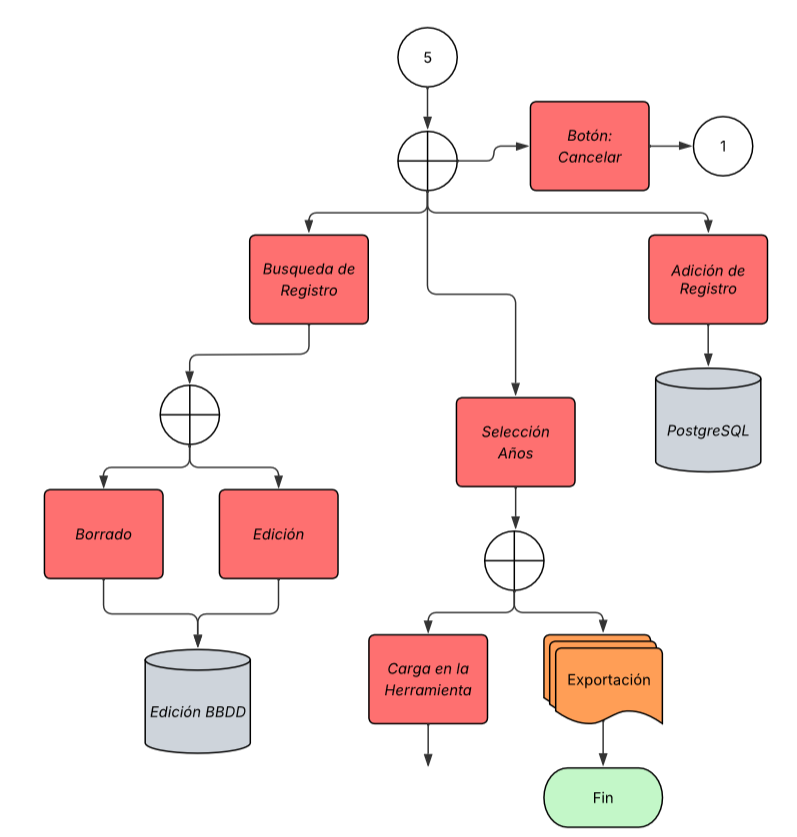
\includegraphics[width=1\textwidth]{img/bbdd.png}
    		\caption{Diagrama de flujo - Interfaz de la \textit{BBDD}.}
    		\label{fig:bbdd}
	\end{figure}
    
\end{itemize}

\subsection{Control de Versiones}
Para el desarrollo del \textit{software} se ha seguido una metodología iterativa e incremental, apoyada en el sistema de control de versiones \textit{Git} y alojada en un repositorio de \textit{GitHub}. A lo largo del ciclo de vida del proyecto, la plataforma ha evolucionado a través de varias versiones principales (ej. Releases v1.0, v2.0 y v3.0), añadiendo en cada iteración mayor robustez al motor matemático y nuevas funcionalidades a la interfaz gráfica. Los diagramas mostrados hacen referencia a las últimas versiones desarrolladas que permiten alcanzar la estabilidad de la arquitectura final.

\section{Arquitectura de Despliegue en Entorno Hospitalario (\textit{HUBU})}
El despliegue de la ``Calculadora de Indicadores'' se ha diseñado siguiendo una arquitectura de \textit{microservicios} basada en contenedores, optimizada para integrarse de forma segura en la infraestructura interna de un centro sanitario (\textit{intranet}). Este modelo garantiza el aislamiento de la aplicación, la seguridad de los datos clínicos y la facilidad de mantenimiento. Este despliegue requiere de un código alternativo al que se va a explicar mas adelante siendo accesible en el siguiente enlace: \href{https://github.com/ngg1017/TFG-2026-Nicolas-Garcia-Gomez-Produccion}{TFG-2026-Nicolas-Garcia-Gomez-Produccion}. La arquitectura se divide en tres capas funcionales descritas a continuación y representadas en el siguiente esquema \ref{fig:esquema_docker}:

\begin{figure}[H]
	\centering
    	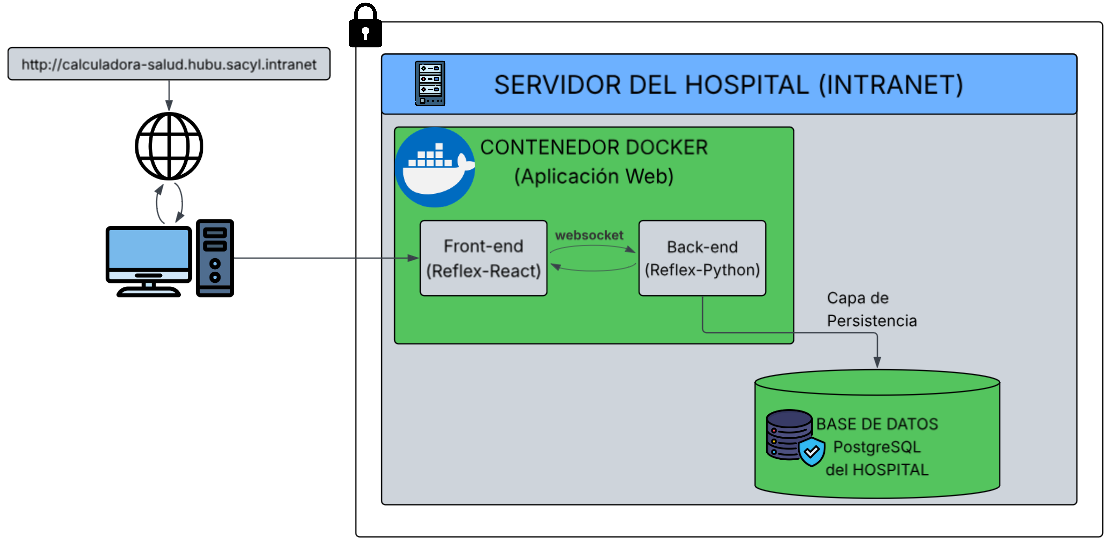
\includegraphics[width=1.3\textwidth]{img/esquema_docker.png}
    	\caption{Arquitectura de Despliegue.}
    	\label{fig:esquema_docker}
\end{figure}

\begin{enumerate}
	\item \textbf{Capa de Acceso de Usuarios (Cliente):} El personal médico accede a la herramienta de forma transparente a través de un navegador \textit{web} estándar, utilizando una \textit{URL} interna proporcionada por la red del hospital (ej. \texttt{http://calculadora-salud.hubu.sacyl.intranet}). Este enfoque \textit{zero-install} elimina la necesidad de instalar \textit{software} local en los equipos de las consultas, centralizando las actualizaciones y reduciendo los puntos de vulnerabilidad. Las peticiones se dirigen a los puertos estándar del servidor del hospital.
	
	\item \textbf{Capa de Aplicación (Contenedor \textit{Docker}\footnote{Permite empaquetar una aplicación con todo lo necesario (código, dependencias, librerías) para que funcione de manera idéntica en cualquier servidor o máquina.}):} El núcleo lógico y visual de la calculadora reside en un único contenedor \textit{Docker} alojado en el \textbf{Servidor del Hospital}. Este contenedor aísla el entorno de ejecución y encapsula las dos piezas fundamentales del \textit{framework Reflex}:
	\begin{itemize}
		\item \textbf{\textit{Frontend} (\textit{Reflex-React}):} Encargado de renderizar la interfaz de usuario de forma reactiva.
		\item \textbf{\textit{Backend} (\textit{Reflex-Python}):} Encargado de procesar la lógica de negocio, las validaciones de grado clínico y la limpieza de datos.
		\item Ambos componentes se comunican en tiempo real mediante un puente virtual interno, implementado a través del \textit{WebSockets}, garantizando una latencia mínima en la interacción.
	\end{itemize}
	
	\item \textbf{Capa de Persistencia de Datos (\textit{PostgreSQL}):} Para el almacenamiento robusto de los registros médicos, la aplicación no utiliza bases de datos volátiles ni locales dentro del contenedor. En su lugar, el \textit{backend} de \textit{Python} establece una conexión directa con la base de datos \textit{PostgreSQL} oficial gestionada por el hospital.
	\begin{itemize}
		\item \textbf{Seguridad de Credenciales:} Para cumplir con el\textbf{ Esquema Nacional de Seguridad (\textit{ENS})} \cite{ens} y las normativas de protección de datos, las credenciales de acceso a la base de datos no están codificadas en el código fuente. Se inyectan de forma segura en el contenedor en el momento del arranque mediante variables de entorno.
		
		\item \textbf{Integración \textit{ORM\footnote{Capa de abstracción que traduce dinámicamente los objetos y funciones de Python en consultas seguras de PostgreSQL, eliminando la necesidad de escribir código SQL nativo.}}:} Las operaciones de lectura, escritura y auditoría se realizan utilizando el \textit{ORM} integrado, lo que previene ataques y asegura la coherencia e integridad de los tipos de datos introducidos por los facultativos.
	\end{itemize}
\end{enumerate}

\section{Arquitectura de Despliegue en Entorno Local}
Para las fases de desarrollo, validación técnica y demostración de la ``Calculadora de Indicadores'', se ha diseñado una arquitectura de despliegue local ejecutada sobre un ordenador personal. Este modelo replica fielmente la lógica del entorno de producción hospitalario mediante tecnología de contenedores, pero condensa los servicios para permitir una ejecución autónoma y controlada. La arquitectura se divide en tres capas funcionales representadas en el siguiente esquema \ref{fig:esquema_docker_pc}:

\begin{figure}[H]
	\centering
    	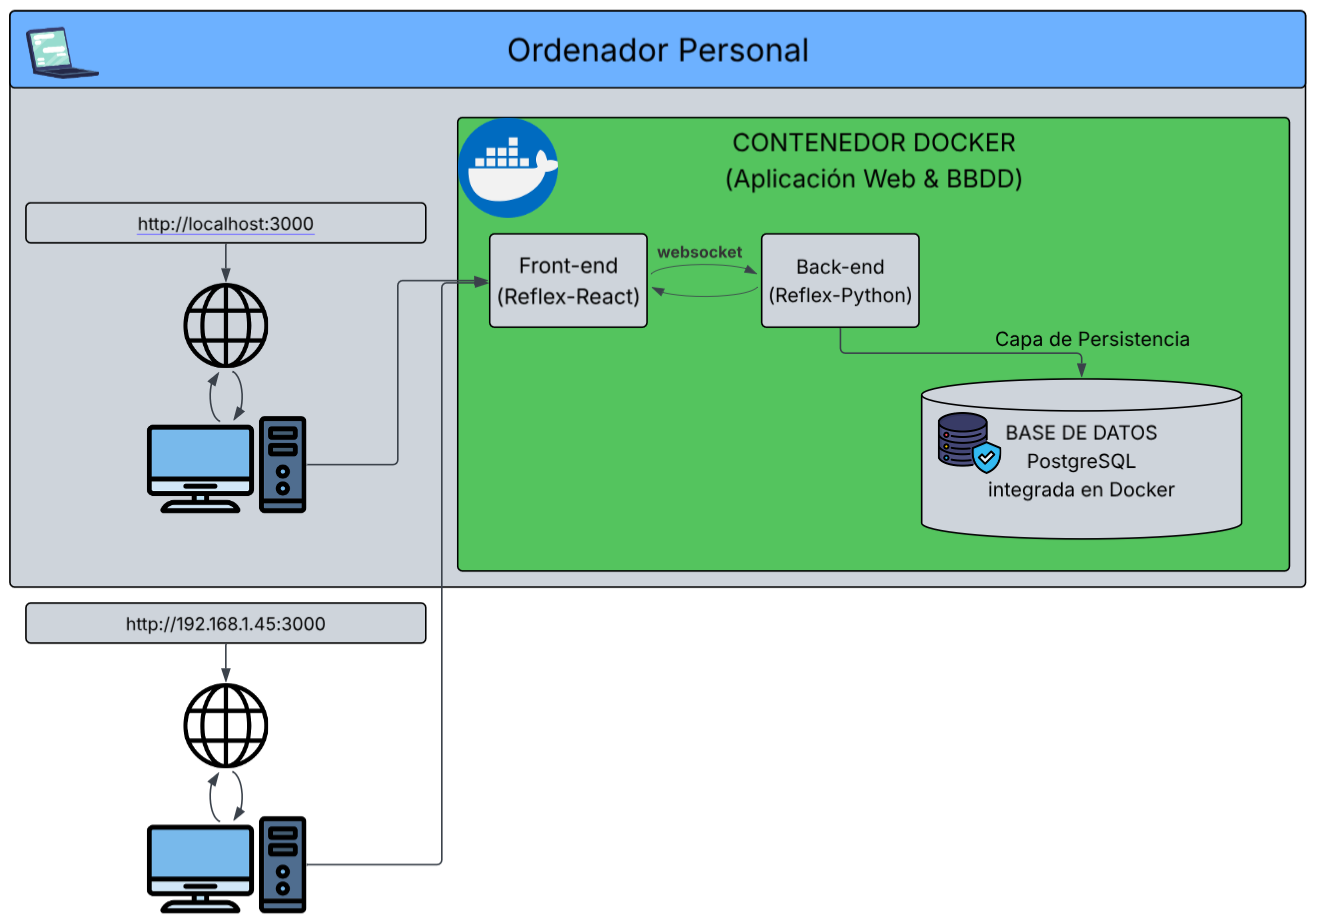
\includegraphics[width=1.3\textwidth]{img/esquema_docker_pc.png}
    	\caption{Arquitectura de Despliegue en Entorno Local.}
    	\label{fig:esquema_docker_pc}
\end{figure}

\begin{enumerate}
	\item \textbf{Capa de Acceso de Usuarios (Cliente):} En este entorno, el acceso a la interfaz se realiza a través de un navegador \textit{web} estándar. Al tratarse de una implementación local, existen dos vías de acceso principales:
	\begin{itemize}
		\item \textbf{Acceso Local (\textit{Loopback\footnote{Término que se utiliza en diferentes áreas de la tecnología para describir un proceso en el que una señal o dato se envía de vuelta a su origen.}}):} Desde el propio equipo anfitrión donde se ejecutan los contenedores, utilizando la dirección \texttt{http://localhost:3000}.
		\item \textbf{Acceso en Red Local (\textit{LAN}):} Desde otros dispositivos autorizados conectados a la misma red (como una \textit{tablet} médica o portátil de planta), introduciendo la dirección \textit{IP} privada del equipo (ej. \texttt{http://192.168.1.45:3000}).
	\end{itemize}
	
	\item \textbf{Capa de Aplicación (Contenedor \textit{Docker}):} El núcleo de la aplicación se ejecuta de forma aislada dentro de un contenedor. Este encapsula las dos piezas fundamentales del \textit{framework Reflex}.
	
	\item \textbf{Capa de Persistencia de Datos (\textit{PostgreSQL} Integrada):} A diferencia del entorno hospitalario, donde la base de datos es externa y gestionada por el centro, en el entorno de pruebas el motor de \textit{PostgreSQL} se despliega de forma integrada en el ecosistema \textit{Docker} del equipo.
	\begin{itemize}
		\item \textbf{Aislamiento y Pruebas de Estrés:} Esta configuración permite disponer de un entorno de datos controlado para realizar migraciones de tablas (\textit{Alembic}), pruebas de carga y simulaciones de ingesta de archivos \textit{CSV} sin riesgo de alterar sistemas externos o comprometer datos reales.
		
		\item \textbf{Integración \textit{ORM}}: El \textit{backend} interactúa con esta base de datos local de forma transparente, asegurando que el código desarrollado sea idéntico al que se utilizará finalmente en la infraestructura del hospital.
	\end{itemize}
\end{enumerate}

\section{Arquitectura de Despliegue en Terminal Portátil (\textit{Raspberry Pi})}
Como variante orientada a la movilidad y la autonomía asistencial, se ha diseñado un despliegue específico sobre un dispositivo \textit{Raspberry Pi}. Esta arquitectura está optimizada para funcionar como un terminal de diagnóstico rápido o ``punto de atención'', donde prima la inmediatez y la sencillez de uso sobre la persistencia de datos a largo plazo. A diferencia de los modelos anteriores, esta configuración prescinde de un motor de base de datos relacional, operando en un modo de análisis volátil. Este despliegue requiere de un código alternativo siendo accesible en el siguiente enlace: \href{https://github.com/ngg1017/TFG-2026-Nicolas-Garcia-Gomez-Portatil}{TFG-2026-Nicolas-Garcia-Gomez-Portatil} y su arquitectura se representa en el siguiente esquema \ref{fig:esquema_docker_portatil}.

\begin{figure}[H]
	\centering
    	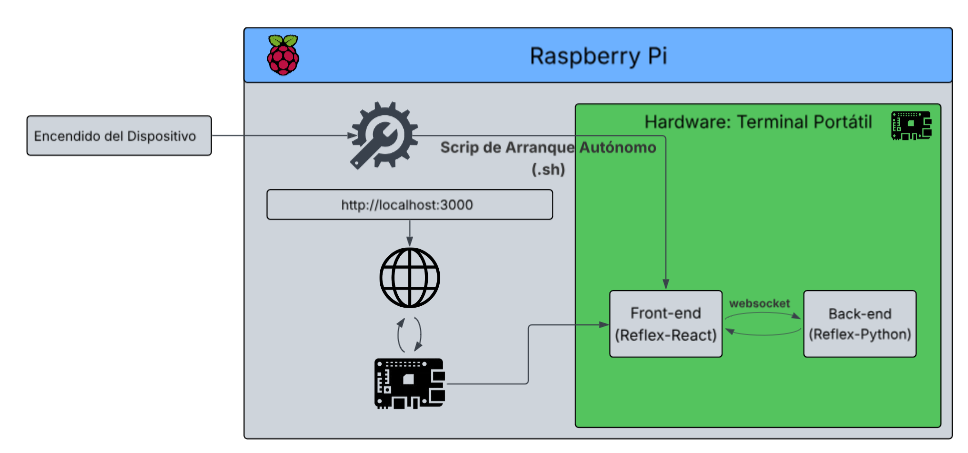
\includegraphics[width=1.1\textwidth]{img/esquema_docker_portatil.png}
    	\caption{Arquitectura de Despliegue en Entorno Portátil.}
    	\label{fig:esquema_docker_portatil}
\end{figure}

\begin{enumerate}
	\item \textbf{Automatización y Gestión del Ciclo de Vida (\textit{Script .sh}):} Para garantizar una experiencia de usuario \textit{Plug \& Play}, el sistema cuenta con un proceso de arranque automatizado. Mediante un \textit{script} de \textit{shell} (\texttt{.sh})\cite{shell} configurado en el gestor de servicios del sistema operativo (\textit{Raspberry Pi OS}), la aplicación se inicia de forma transparente al encender el dispositivo. Este \textit{script} se encarga de:
	\begin{itemize}
		\item Verificar la integridad del entorno virtual de \textit{Python}.
		\item Levantar los servicios de \textit{Frontend} y \textit{Backend} sin intervención humana.
		\item Lanzar el navegador nativo en modo ``kiosco'' (pantalla completa) apuntando a la dirección local.
	\end{itemize}
	
	\item \textbf{Procesamiento Efímero y Análisis en Memoria (\textit{RAM}):} En esta arquitectura, la aplicación opera de forma puramente transaccional. El flujo de trabajo se centra exclusivamente en la subida de archivos \textit{CSV} por parte del facultativo. 
	\begin{itemize}
		\item Los datos se cargan directamente en la memoria \textit{RAM} del dispositivo para su procesamiento estadístico instantáneo.
		\item Se mantiene la potencia analítica completa del motor de \textit{Python}, permitiendo la generación de gráficas de control y el cálculo de indicadores de seguridad en tiempo real.
	\end{itemize}
	
	\item \textbf{Gestión de Datos sin Persistencia:} Al no contar con una capa de base de datos (\textit{PostgreSQL}), el sistema garantiza la máxima privacidad de la información clínica en entornos fuera de la \textit{intranet} hospitalaria segura. Una vez finalizada la sesión o reiniciado el dispositivo, los datos procesados desaparecen de la memoria volátil. 
	\begin{itemize}
		\item Este enfoque elimina los riesgos de seguridad física asociados al robo o pérdida del dispositivo portátil, ya que no se almacena información sensible en el disco de la \textit{Raspberry Pi}.
		\item El resultado final del análisis puede ser exportado por el médico mediante la generación del informe \textit{PDF}, sirviendo este como el único entregable permanente de la sesión.
	\end{itemize}
\end{enumerate}

En este apartado se incluye una breve descripción de todos los componentes \textit{hardware} utilizados.

\begin{itemize}
    \item \textbf{\textit{Raspberry Pi 3 model B}:} (Figura \ref{fig:raspberrypi}) Es un ordenador de placa única (\textit{SBC}) de bajo coste y tamaño reducido (como una tarjeta de crédito), creado por la \textit{Raspberry Pi Foundation} en 2012 para promover la enseñanza de la informática. Ejecuta \textit{Linux}, cuenta con puertos \textit{USB}, \textit{HDMI}, \textit{Wi-Fi} y pines \textit{GPIO} perfectos para este tipo de proyectos.
    
    \begin{figure}[h]
        \centering
        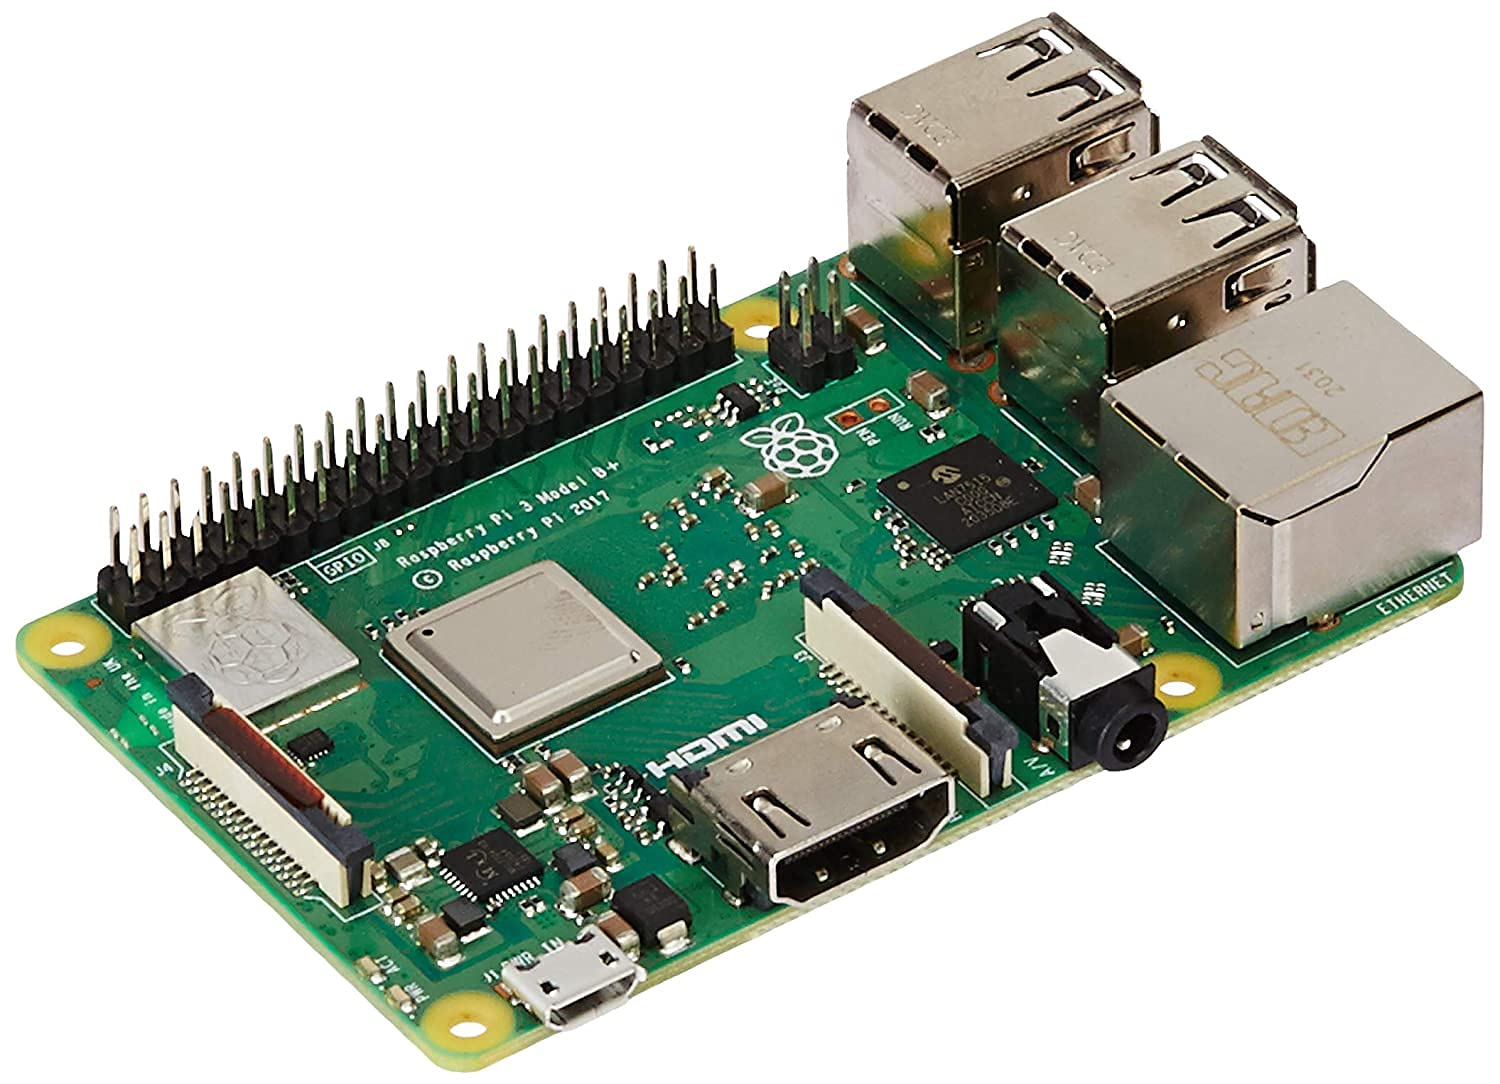
\includegraphics[width=0.7\textwidth]{img/raspberrypi.jpg}
        \caption{Raspberry Pi 3 model B. \cite{raspberryC}}
        \label{fig:raspberrypi}
    \end{figure}
    
    \item \textbf{\textit{Pantalla Raspberry Pi LCD 7'' Táctil}:} (Figura \ref{fig:pantalla}) Es un dispositivo de \textbf{800 x 480} con el que convertir una \textit{Raspberry Pi} en una \textit{tablet} generando en un sistema totalmente interactivo. Esta pantalla táctil utiliza \textit{drivers} que funcionan con toques de diez dedos, y también puede mostrar un teclado en pantalla.

    \begin{figure}[h]
        \centering
        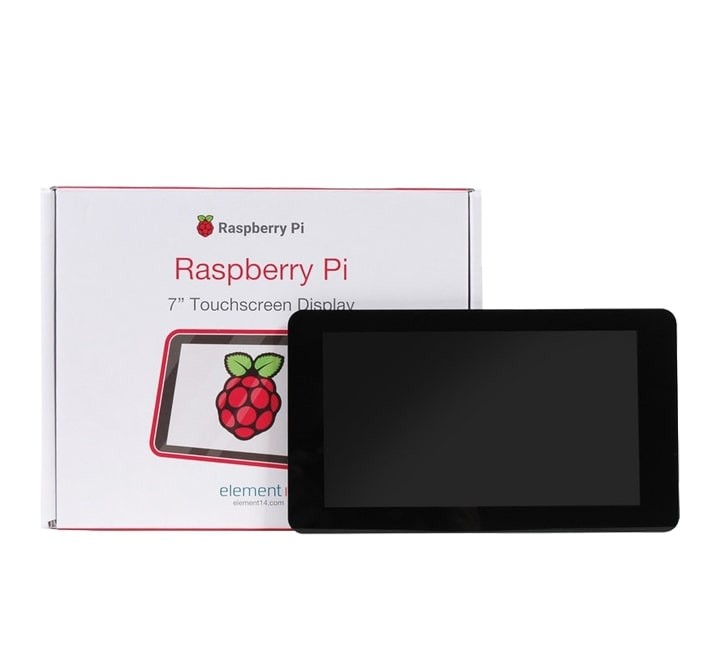
\includegraphics[width=0.7\textwidth]{img/pantalla.jpg}
        \caption{Pantalla Raspberry Pi LCD 7'' Táctil. \cite{pantalla}}
        \label{fig:pantalla}
    \end{figure}
    
    \item \textbf{\textit{Sandisk MicroSD Ultra 32GB}:} (Figura \ref{fig:sd}) Es un dispositivo de almacenamiento de datos portátil y extremadamente pequeño basado en tecnología \textit{flash}, utilizado para almacenar el \textit{SO} de la \textit{RaspBerry Pi}.

    \begin{figure}[h]
        \centering
        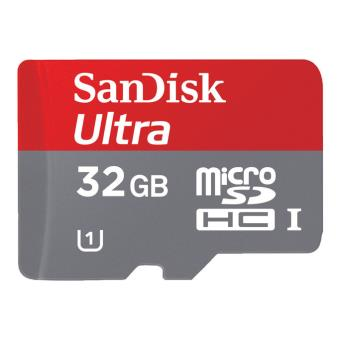
\includegraphics[width=0.3\textwidth]{img/sd.jpg}
        \caption{MicroSD 32GB. \cite{sd}}
        \label{fig:sd}
    \end{figure}

    \item \textbf{Cables:} El cableado necesario para realizar las conexiones pertinentes.

    \item \textbf{Caja para prototipos:} (Figura \ref{fig:caja}) Almacena todo el \textit{hardware} necesario para el funcionamiento del prototipo. Fabricada mediante la impresión \textit{3D}\footnote{Es un proceso que crea objetos tridimensionales sólidos capa por capa a partir de un modelo digital.} resistente que protegerá el microprocesador y las conexiones entre todos los componentes.

    \begin{figure}[h]
        \centering
        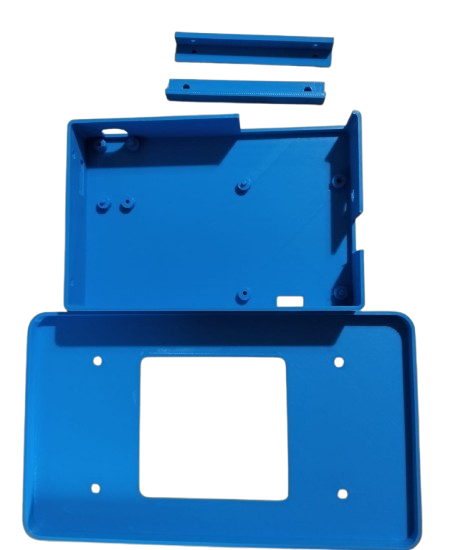
\includegraphics[width=0.5\textwidth]{img/carcasa.png}
        \caption{Caja de componentes. \cite{carcasa}}
        \label{fig:caja}
    \end{figure}
    
    \item \textbf{\textit{Adafruit PowerBoost 1000C}\footnote{Durante la fase de validación física del prototipo, se ha determinado empíricamente que módulos de batería como el \textit{Adafruit PowerBoost 1000C} resultan insuficientes para soportar el consumo combinado de la \textit{Raspberry Pi} y el panel táctil de 7 pulgadas. Superar su carga nominal provoca un estrés térmico en el módulo que puede derivar en picos de tensión y causar daños eléctricos irreversibles en la placa controladora de la pantalla. Por consiguiente, para garantizar la integridad y estabilidad del \textit{hardware} en entornos de producción, es un requisito estricto sustituir este componente por un sistema de alimentación ininterrumpida (tipo \textit{UPS}) diseñado para proporcionar una salida continua y estable de, al menos, 5\textit{V} y 3 Amperios.}:} (Figura \ref{fig:adafruit}) Es un módulo versátil de gestión de energía (convertidor \textit{DC/DC boost}) con cargador integrado, diseñado para alimentar proyectos portátiles. Convierte el voltaje de baterías \textit{LiIon/LiPoly} de 3,7\textit{V} a una salida estable de 5,2\textit{V} \textit{DC}, ideal para dispositivos como \textit{Arduino} o \textit{Raspberry Pi}, permitiendo la carga de la batería y la alimentación del proyecto simultáneamente.

    \begin{figure}[h]
        \centering
        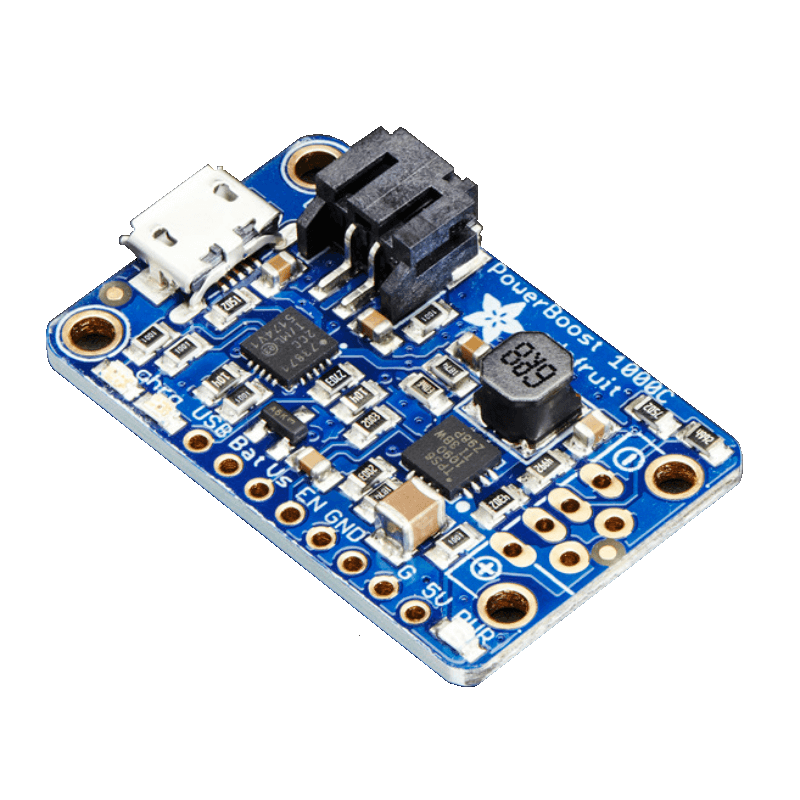
\includegraphics[width=0.3\textwidth]{img/adafruit.png}
        \caption{\textit{Adafruit PowerBoost 1000C}. \cite{adafruit}}
        \label{fig:adafruit}
    \end{figure}
    
    \item \textbf{Batería de 6000\textit{mAH} a 3,7\textit{V}:} (Figura \ref{fig:bateria}) Almacena la energía en forma química para posteriormente convertirla en energía eléctrica para el suministro de corriente a diversos equipos y sistemas.

    \begin{figure}[h]
        \centering
        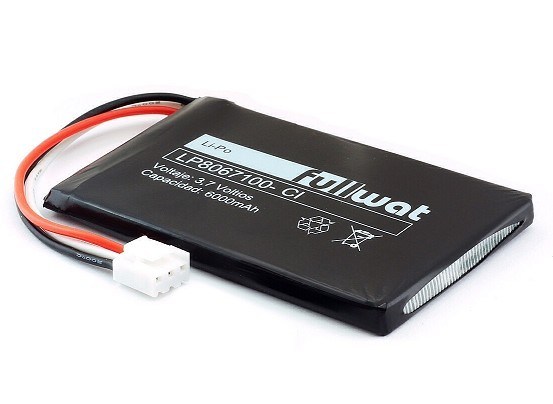
\includegraphics[width=0.3\textwidth]{img/bateria.jpg}
        \caption{Batería de 6000 \textit{mAH} a 3,7\textit{V}. \cite{bateria}}
        \label{fig:bateria}
    \end{figure}
    
    \item \textbf{Interruptor \textit{SPDT}:} (Figura \ref{fig:interruptor}) Es un componente eléctrico con tres terminales: uno común (entrada) y dos de salida. Permite dirigir la corriente entre dos trayectorias distintas, en este proyecto solo se necesita una de las trayectorias; sin embargo, en el proveedor de compra los interruptores  \textit{SPST}\footnote{Es el tipo más básico de interruptor eléctrico, diseñado para abrir o cerrar un único circuito} no se encontraban disponibles.

    \begin{figure}[h]
        \centering
        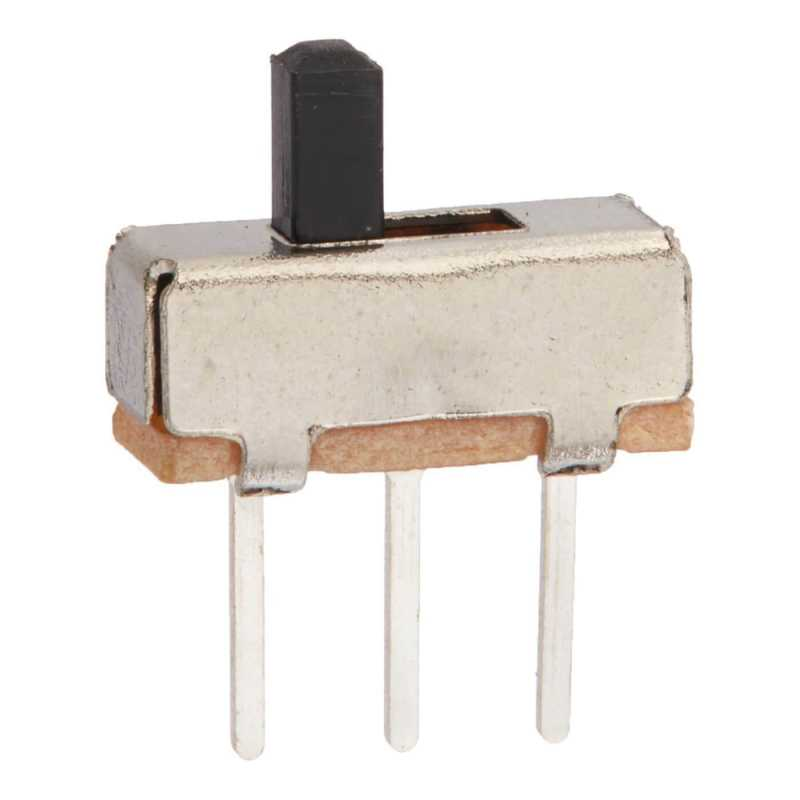
\includegraphics[width=0.2\textwidth]{img/interruptor.jpg}
        \caption{Interruptor \textit{SPDT}. \cite{interruptor}}
        \label{fig:interruptor}
    \end{figure}
\end{itemize}

La elección de la \textit{Raspberry Pi} frente a otros sistemas informáticos convencionales o terminales industriales para el diseño del dispositivo físico se justifica en los siguientes factores:

\begin{enumerate}
    \item \textbf{Disipación térmica pasiva (Asepsia clínica):} Al utilizar un \textit{SoC} altamente eficiente, la placa carece de ventiladores mecánicos para su refrigeración. Este atributo de \textit{hardware} es crítico en un entorno de aislamiento como la \textit{URCCPQ}, ya que elimina la generación de corrientes de aire que podrían dispersar polvo o patógenos aerógenos, contribuyendo a la esterilidad del área.
    \item \textbf{Eficiencia energética y autonomía:} Su arquitectura \textit{ARM} presenta un consumo eléctrico drásticamente inferior al de los procesadores \textit{x86/x64} convencionales. Esto permite que el terminal sea alimentado de forma estable y prolongada mediante baterías externas estándar, un requisito físico indispensable para garantizar la portabilidad de la ``\textit{tablet} médica''.
    \item \textbf{Factor de forma y empaquetado (\textit{SBC}):} Al tratarse de un ordenador de placa única (\textit{Single Board Computer}), concentra la \textit{CPU}, memoria e interfaces de red en dimensiones muy reducidas (formato tarjeta de crédito). Esto ha permitido integrarla de forma compacta en la carcasa del dispositivo portátil sin comprometer la ergonomía.
    \item \textbf{Interfaces físicas nativas:} La placa incorpora de fábrica conectividad directa para pantallas táctiles (mediante puertos \textit{DSI} o \textit{micro-HDMI}) y pines de entrada/salida (\textit{GPIO}), lo que facilita el ensamblaje directo de la pantalla interactiva sin requerir tarjetas controladoras adicionales ni cableado voluminoso.
\end{enumerate}
